\documentclass[tikz, border=2pt]{standalone}

\usepackage{amsmath,amssymb}
\usepackage{pgfplots}
\pgfplotsset{compat=1.18}
\usepackage{xcolor}

\definecolor{utnblue}{RGB}{0, 51, 102}
\definecolor{utnred}{RGB}{204, 0, 0}

\begin{document}
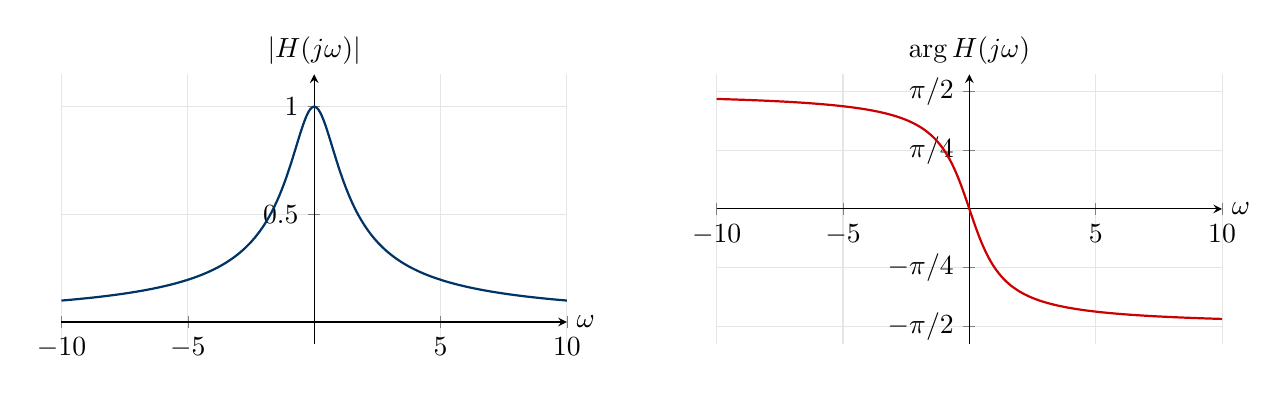
\begin{tikzpicture}

% --- Módulo ---
\begin{axis}[
    name=mod,
    width=8cm, height=5cm,
    xmin=-10, xmax=10,
    ymin=-0.1, ymax=1.15,
    xlabel={$\omega$},
    ylabel={$|H(j\omega)|$},
    axis lines=middle,
    enlargelimits=false,
    grid=major,
    grid style={gray!20},
    every axis x label/.style={at={(ticklabel* cs:1)}, anchor=west},
    every axis y label/.style={at={(ticklabel* cs:1)}, anchor=south},
]
\addplot[utnblue, thick, samples=300, domain=-10:10]
    ({x}, {1/sqrt(1+x^2)});
\end{axis}

% --- Fase ---
\begin{axis}[
    at={(mod.right of east)}, anchor=left of west, xshift=1.0cm,
    width=8cm, height=5cm,
    xmin=-10, xmax=10,
    ymin=-1.8, ymax=1.8,
    ytick={-1.5708, -0.7854, 0, 0.7854, 1.5708},
    yticklabels={$-\pi/2$, $-\pi/4$, $0$, $\pi/4$, $\pi/2$},
    xlabel={$\omega$},
    ylabel={$\arg H(j\omega)$},
    axis lines=middle,
    enlargelimits=false,
    grid=major,
    grid style={gray!20},
    every axis x label/.style={at={(ticklabel* cs:1)}, anchor=west},
    every axis y label/.style={at={(ticklabel* cs:1)}, anchor=south},
]
\addplot[utnred, thick, samples=300, domain=-10:10]
    ({x}, {-rad(atan(x))});
\end{axis}

\end{tikzpicture}
\end{document}
